\documentclass{article}
\usepackage[utf8]{inputenc}
\usepackage{pgfplots}
\pgfplotsset{width=10cm,compat=1.9}
\usepackage{amsmath,amssymb,amsthm}
\usepackage{graphicx}
\usepackage{float}
\usepackage{blindtext}
\usepackage{hyperref}
\usepackage{verbatim}
\usepackage{gensymb}
\usepackage{enumerate}
\usepackage{xcolor}
\usepackage{graphicx}
\hypersetup{
    colorlinks=true,
    linkcolor=blue,
    filecolor=magenta,      
    urlcolor=cyan,
    pdftitle={Overleaf Example},
    pdfpagemode=FullScreen,
    }
\usepackage[slovene]{babel}

\setlength{\parindent}{0pt}
\setlength{\parskip}{4pt}

\newcounter{example}[section]
\newenvironment{example}[1][]{\refstepcounter{example}\par\medskip
   \noindent \textbf{Naloga~\theexample. #1} \rmfamily}{\medskip}

\newtheorem*{zgled}{Zgled}

\title{Funkcije}
\author{Bor Bregant}
\date{\vspace{-5ex}}

\begin{document}

\thispagestyle{empty}	% ne oštevilči strani

\noindent MATEMATIKA, \quad 4. A \hfill Škofijska klasična gimnazija
\hrule
\vspace{1ex}
\noindent \textbf{Tema:} Kompozitum funkcij
\vspace{1ex}

\noindent \textbf{Enota:} Funkcije
\vspace{1ex}

\noindent \textbf{Datum:} 23. 11. 2023
\vspace{1ex}

\noindent \textbf{Mentorica:} dr. Marina Rugelj
\vspace{1ex}

\noindent \textbf{Viri in literatura:} Tempus novum, 2020, Pavlič G. in drugi
\vspace{1ex}
\hrule
\vspace{2ex}
\noindent \textbf{Učne oblike:} Frontalna, individualna
\vspace{1ex}

\noindent \textbf{Učne metode:} Razlaga
\vspace{1ex}

\noindent \textbf{Učni pripomočki:} Tabla, učbenik
\vspace{1ex}

\noindent \textbf{Učni cilji:} Dijaki/dijakinje uporablja ter obravnava kompozitume funkcij, ter s to operacijo računa.
\vspace{4ex}
\hrule
\vspace{5ex}
\noindent \textbf{Vsebina in potek:} 

\vspace{5ex}

\section*{\textcolor{violet}{Uvodna motivacija}}

\textbf{\textcolor{violet}{V razpravi razmišljamo, kako lahko funkcije med sabo zaporedno sestavljamo}}

\textbf{\textcolor{violet}{Formalna definicija s tabelno sliko}}

\subsection*{Kompozitum funkcij}

\begin{figure}[H]
    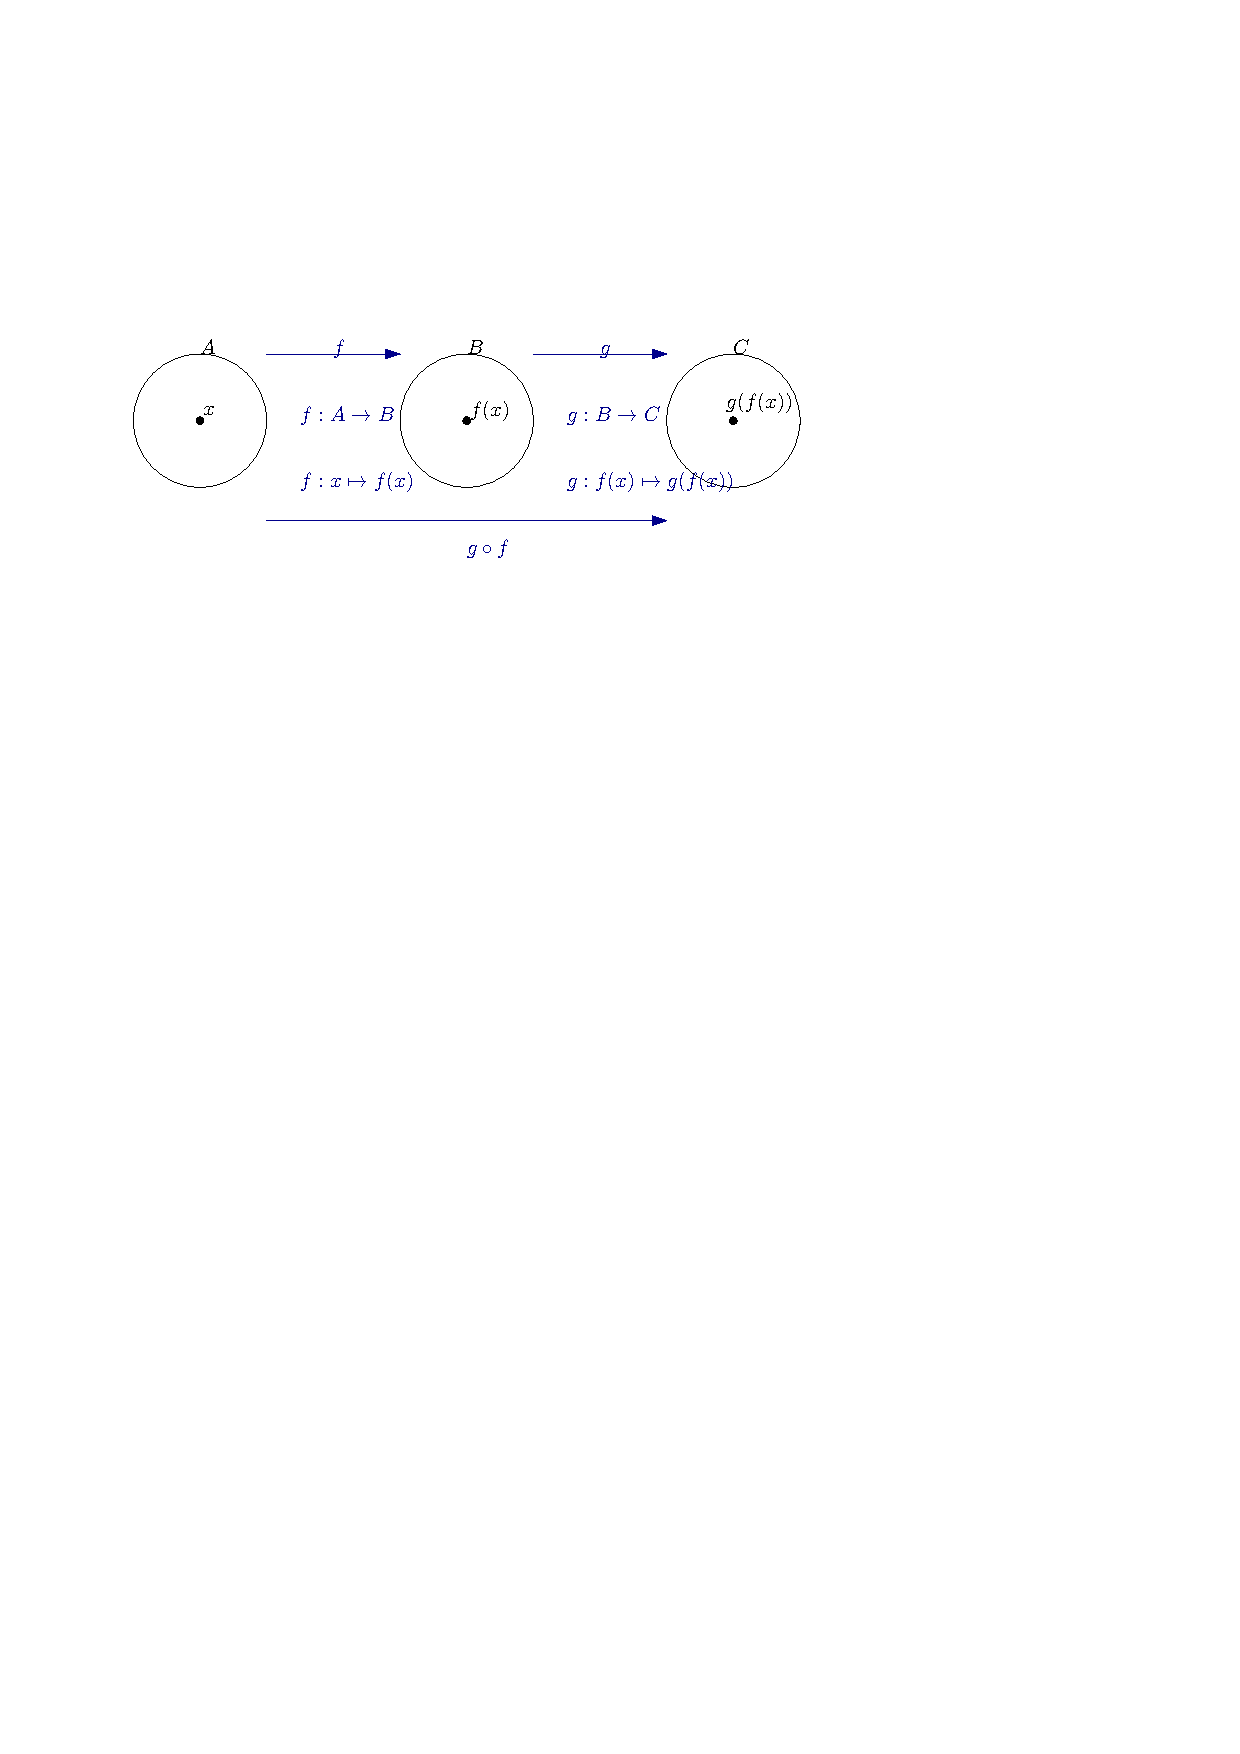
\includegraphics[width=0.7\textwidth]{kompozitum.pdf}
    \centering
\end{figure}

\begin{align*}
    & g\circ f: A\rightarrow C\\
    & g\circ f: x\mapsto g(f(x))\\
    & (g\circ f)(x)=g(f(x))\\
\end{align*}

\textbf{\textcolor{violet}{Dijaki pred tablo rešujejo naslednje naloge. Če gre dobro, lahko delajo individualno ali pa v tandemu.}}

\begin{zgled}
    Izračunaj $f\circ g$ in $g\circ f$ za $f(x)=\ln (x^2+2)$ in $g(x)=3x-1$ in pokaži, da ta operacija ni komutativna.
\end{zgled}

\begin{zgled}
    Poišči inverzno funkcijo za $f(x)=\sqrt[3]{x}+1$ in pokaži, da velja $(f\circ f^{-1})(x)=(f^{-1}\circ f)(x)=x$.
\end{zgled}
   
\begin{zgled}
    Dani sta funkciji $f(x)=2x-3$ in $g(x)=-x+2$. Za katera realna števila $x$ je $f(2x)=g(x)$ in za katera $f(-2)=g(x^2)$.
\end{zgled}

\begin{zgled}
    Dani sta funkciji $f(x)=3x+2$ in $g(x)=2x+n$. Za katera števila $n$ velja $f(g(x))=g(f(x))$?
\end{zgled}

\begin{zgled}
    Določi $k$, da bo $f(g(x))=g(f(x))$, kjer $f(x)=kx+3$ in $g(x)=kx-1$.
\end{zgled}

\begin{example}
    Domača naloga 574, 573ace, 587, 592ac
\end{example}

\textbf{\textcolor{violet}{Dijaki si DN zabeležijo in odidejo iz razreda}}

\end{document}
